
% ==========================================
% KAPITEL 4: IMPLEMENTIERUNG & PHYSIKALISCHER KERN
% ==========================================
\section{Physikalischer Kern und Implementierung}
\label{sec:implementierung}

Der rechnerische Kern der Physik-Engine basiert auf robuster linearer Algebra, um Randkollisionen zu lösen. Um den Rechendurchsatz bei Millionen von Strahlen zu maximieren, verzichtet die Engine auf rechnerisch aufwändige trigonometrische Funktionen zugunsten reiner Vektormathematik.

\subsection{2D-Strahlensegmentschnitt}
\label{subsec:2d_schnitt}

\paragraph{Geometrische Definitionen}
Ein Schallstrahl wird durch einen Ursprungspunkt $O$ und einen normalisierten Richtungsvektor definiert $\vec{D}$. Jeder Punkt $P$ entlang der Strahlenbahn kann als Funktion der skalaren Distanz $t$ berechnet werden: $P(t) = O + t\vec{D}$.
Eine Wand wird als Liniensegment dargestellt, definiert durch zwei Endpunkte $A$ und $B$. Mit dem Wandvektor $\vec{V} = B - A$ ergibt sich die parametrische Gleichung: $W(u) = A + u\vec{V}$.

\paragraph{Schnittpunktberechnung und Validierung}
Durch das Gleichsetzen der Gleichungen und die Definition der Schnittdeterminante als $\det = \vec{D} \times \vec{V}$ können die Parameter $t$ und $u$ isoliert algebraisch gelöst werden.
Eine physikalische Kollision wird validiert, wenn die Determinante nicht verschwindend gering ist (Ausschluss von Parallelität), die Distanz $t \ge 0$ ist (Ausschluss von Rückwärtstreffern) und der Parameter $0 \le u \le 1$ liegt (Einschränkung auf das Liniensegment).

\paragraph{Vektorreflexion}
Die Richtung des reflektierten Strahls $\vec{R}$ wird bestimmt, indem von der Richtung des einfallenden Strahls $\vec{D}$ das Doppelte der Projektion dieser Richtung auf die Oberflächennormale $\vec{N}$ subtrahiert wird:
\[\vec{R} = \vec{D} - 2(\vec{D} \cdot \vec{N})\vec{N}\]
Innerhalb der Rust-Codebasis wird diese Berechnung durch die \texttt{reflect} Methode des \texttt{glam}-Crates optimiert, die SIMD-Instruktionen für minimalen Overhead nutzt.


\subsection{Umstellung auf 3D: \texttt{Vec3} und Möller-Trumbore-Algorithmus}
\label{subsec:3d_migration}

Die aktuelle Implementierung der Physik-Engine arbeitet vollständig im
dreidimensionalen Raum. Im Vergleich zur ursprünglichen zweidimensionalen
Grundidee mussten dafür insbesondere die geometrischen Datenstrukturen, die
Raummodellierung und die Kollisionsberechnung angepasst werden.

Ziel dieser Umstellung war es, Schallstrahlen nicht mehr ausschließlich in
einer Ebene zu simulieren, sondern ihre Ausbreitung in einem Raum mit Breite,
Tiefe und Höhe abzubilden. Positionen und Richtungen werden daher nicht mehr
mit zwei Koordinaten, sondern mit dem Datentyp \texttt{Vec3} beschrieben. Ein
Punkt im dreidimensionalen Raum besitzt eine \(x\)-, \(y\)- und
\(z\)-Koordinate:

\[
    P = (x,y,z)
\]

Diese Erweiterung betrifft insbesondere die Positionen von Lautsprecher und
Mikrofon, die Ursprünge und Richtungen der Strahlen sowie die berechneten
Reflexionspunkte an den Raumflächen. Während Wände in der zweidimensionalen
Version als Liniensegmente modelliert werden konnten, müssen sie in der
3D-Simulation als Flächen behandelt werden. Die Raumflächen werden deshalb aus
Dreiecken aufgebaut. Zur Berechnung der Schnittpunkte zwischen einem Strahl
und diesen Dreiecken wird der Möller-Trumbore-Algorithmus verwendet.

\subsubsection{Neue 3D-Datenstrukturen: \texttt{Ray} und \texttt{Triangle}}
\label{subsubsec:ray_triangle}

Die Grundlage der Umstellung war die Anpassung der zentralen Datenstrukturen.
Ein Schallstrahl wird in der neuen Implementierung durch die Struktur
\texttt{Ray} beschrieben. Diese enthält den aktuellen Ursprung des Strahls und
seine Richtung im dreidimensionalen Raum:

\begin{lstlisting}[language=Rust]
pub struct Ray {
    pub origin: Vec3,
    pub direction: Vec3,
}
\end{lstlisting}

Der Wert \texttt{origin} beschreibt den aktuellen Startpunkt des Strahls. Zu
Beginn entspricht dieser Punkt der Lautsprecherposition. Nach jeder Reflexion
wird der berechnete Trefferpunkt an einer Fläche zum neuen Ursprung des
reflektierten Strahls. Der Wert \texttt{direction} beschreibt die
Ausbreitungsrichtung. Dieser Richtungsvektor wird normalisiert verwendet, damit
nur seine Richtung und nicht seine Länge eine Rolle spielt.

Auch die Modellierung der Raumflächen musste verändert werden. In der
zweidimensionalen Version konnten Wände als Liniensegmente dargestellt werden.
In einem dreidimensionalen Raum muss ein Strahl jedoch mit Flächen kollidieren.
Aus diesem Grund werden Raumflächen nun als Dreiecke modelliert:

\begin{lstlisting}[language=Rust]
pub struct Triangle {
    pub v0: Vec3,
    pub v1: Vec3,
    pub v2: Vec3,
    pub absorption: f32,
}
\end{lstlisting}

Ein Dreieck besteht aus den drei Eckpunkten \texttt{v0}, \texttt{v1} und
\texttt{v2}. Diese Punkte definieren eindeutig eine Fläche im
3D-Raum. Zusätzlich besitzt jedes Dreieck einen Absorptionswert, der beschreibt,
wie stark ein Schallstrahl bei einer Reflexion an der jeweiligen Fläche
abgeschwächt wird. Damit enthält die Struktur neben der geometrischen
Beschreibung auch eine akustische Eigenschaft.

\subsubsection{Ablösung des 2D-Segment-Schnitts}
\label{subsubsec:replace_2d_intersection}

Der vorherige Schnittpunktalgorithmus war auf zweidimensionale
Strahl-Segment-Schnitte ausgelegt. Dabei wurde geprüft, ob ein Strahl eine
Wandlinie innerhalb eines begrenzten Segments trifft. Dieses Verfahren ist für
einen dreidimensionalen Raum nicht ausreichend, da Wände, Boden und Decke nicht
als Linien, sondern als Flächen betrachtet werden müssen.

Für die 3D-Version wurde daher auf Strahl-Dreieck-Schnittpunkte umgestellt.
Dreiecke eignen sich besonders für diese Aufgabe, da sie stets planar sind und
komplexe Flächen aus mehreren Dreiecken zusammengesetzt werden können. Dadurch
kann die Simulation nicht nur einfache rechteckige Räume, sondern grundsätzlich
auch komplexere polygonale Geometrien verarbeiten.

\subsubsection{Aufbau des 3D-Raums aus Dreiecken}
\label{subsubsec:room_triangles}

Obwohl der Schnittpunktalgorithmus mit Dreiecken arbeitet, bestehen einfache
Raumflächen wie Boden, Decke oder Wände meistens aus Rechtecken. Deshalb wird
jede rechteckige Raumfläche in zwei Dreiecke zerlegt. Dies geschieht in der
Hilfsfunktion \texttt{add\_rect\_as\_two\_triangles}:

\begin{lstlisting}[language=Rust]
fn add_rect_as_two_triangles(
    triangles: &mut Vec<Triangle>,
    a: Vec3,
    b: Vec3,
    c: Vec3,
    d: Vec3,
    absorption: f32,
) {
    triangles.push(Triangle {
        v0: a,
        v1: b,
        v2: c,
        absorption,
    });

    triangles.push(Triangle {
        v0: a,
        v1: c,
        v2: d,
        absorption,
    });
}
\end{lstlisting}

Das erste Dreieck besteht aus den Punkten \texttt{a}, \texttt{b} und
\texttt{c}. Das zweite Dreieck besteht aus den Punkten \texttt{a}, \texttt{c}
und \texttt{d}. Zusammen bilden beide Dreiecke wieder die vollständige
rechteckige Fläche. Dadurch kann der Möller-Trumbore-Algorithmus einheitlich auf
alle Raumflächen angewendet werden.

Im Hauptprogramm wird zunächst eine Liste für alle Dreiecke des Raums angelegt:

\begin{lstlisting}[language=Rust]
let mut room: Vec<Triangle> = Vec::new();
\end{lstlisting}

Anschließend werden Boden, Decke und die vier Wände des Testraums hinzugefügt.
Der Raum besitzt im Testaufbau eine Breite von \(10{,}0\), eine Tiefe von
\(10{,}0\) und eine Höhe von \(3{,}0\). Das Koordinatensystem ist so aufgebaut,
dass \(x\) die horizontale Richtung, \(y\) die Tiefe des Raums und \(z\) die
Höhe beschreibt. Ein Beispiel ist der Boden des Raums:

\begin{lstlisting}[language=Rust]
add_rect_as_two_triangles(
    &mut room,
    Vec3::new(0.0, 0.0, 0.0),
    Vec3::new(width, 0.0, 0.0),
    Vec3::new(width, depth, 0.0),
    Vec3::new(0.0, depth, 0.0),
    absorption,
);
\end{lstlisting}

Alle vier Punkte besitzen hier die \(z\)-Koordinate \(0{,}0\), da sich der
Boden auf der Höhe null befindet. Für die Decke wird dagegen die
\(z\)-Koordinate \texttt{height} verwendet. Bei den Wänden bleibt jeweils eine
Koordinate konstant, während die beiden anderen Koordinaten die jeweilige
Wandfläche aufspannen.

\subsubsection{Möller-Trumbore-Algorithmus}
\label{subsubsec:moller_trumbore}

Zur Berechnung von Strahl-Dreieck-Schnittpunkten wurde der
Möller-Trumbore-Algorithmus \parencite{moeller1997} implementiert. Dieser Algorithmus wird häufig im
Raytracing verwendet, da er direkt prüft, ob ein Strahl ein Dreieck trifft, ohne
zuvor explizit die Ebenengleichung des Dreiecks bestimmen zu müssen.

Die Funktion \texttt{check\_intersection} bildet den Kern dieser
Schnittpunktprüfung. Sie erhält einen Strahl und ein Dreieck. Falls ein gültiger
Treffer existiert, gibt sie einen neuen reflektierten Strahl zurück. Liegt kein
gültiger Treffer vor, wird \texttt{None} zurückgegeben.

Zunächst werden aus den drei Eckpunkten des Dreiecks zwei Kantenvektoren
berechnet:

\begin{lstlisting}[language=Rust]
let edge1 = triangle.v1 - triangle.v0;
let edge2 = triangle.v2 - triangle.v0;
\end{lstlisting}

Diese beiden Kantenvektoren spannen die Dreiecksfläche im Raum auf.
Anschließend wird ein Kreuzprodukt zwischen der Strahlrichtung und der zweiten
Dreieckskante gebildet:

\begin{lstlisting}[language=Rust]
let h = ray.direction.cross(edge2);
let a = edge1.dot(h);
\end{lstlisting}

Der Wert \texttt{a} zeigt an, ob der Strahl parallel zur Dreiecksfläche
verläuft. Ist dieser Wert nahe null, kann kein eindeutiger Schnittpunkt
berechnet werden. Deshalb wird mit einem kleinen Epsilon-Wert gearbeitet:

\begin{lstlisting}[language=Rust]
let epsilon = 1e-6;

if a.abs() < epsilon {
    return None;
}
\end{lstlisting}

Diese Toleranz ist notwendig, da Gleitkommazahlen nicht immer exakt berechnet
werden. Ohne den Schwellenwert könnten numerische Rundungsfehler zu falschen
Treffern führen.

Anschließend wird die erste baryzentrische Koordinate \(u\) berechnet:

\begin{lstlisting}[language=Rust]
let f = 1.0 / a;
let s = ray.origin - triangle.v0;
let u = f * s.dot(h);

if u < 0.0 || u > 1.0 {
    return None;
}
\end{lstlisting}

Liegt \(u\) außerhalb des Bereichs von \(0{,}0\) bis \(1{,}0\), trifft der
Strahl möglicherweise die Ebene des Dreiecks, aber nicht die begrenzte
Dreiecksfläche selbst. Danach wird die zweite baryzentrische Koordinate \(v\)
berechnet:

\begin{lstlisting}[language=Rust]
let q = s.cross(edge1);
let v = f * ray.direction.dot(q);

if v < 0.0 || u + v > 1.0 {
    return None;
}
\end{lstlisting}

Die Bedingung \(u + v > 1{,}0\) stellt sicher, dass sich der Trefferpunkt nicht
außerhalb des Dreiecks befindet. Ein gültiger Treffer liegt nur dann vor, wenn
die baryzentrischen Koordinaten innerhalb der Dreiecksgrenzen bleiben.

Zum Schluss wird der Parameter \(t\) berechnet. Dieser beschreibt die Entfernung
des Schnittpunkts entlang der Strahlrichtung:

\begin{lstlisting}[language=Rust]
let t = f * edge2.dot(q);

if t < 0.001 {
    return None;
}
\end{lstlisting}

Negative oder sehr kleine Werte werden verworfen, damit Treffer hinter dem
Ursprung oder unmittelbar am Startpunkt nicht berücksichtigt werden. Die
Ursache und die diagnostische Untersuchung solcher Selbsttreffer werden in
Abschnitt~\ref{subsec:epsilon_fix} ausführlicher behandelt.

\subsubsection{Reflexionsberechnung im 3D-Raum}
\label{subsubsec:3d_reflection}

Die zugrunde liegende Reflexionsgleichung entspricht der bereits im
2D-Abschnitt beschriebenen Vektorreflexion. Im dreidimensionalen Fall wird die
Oberflächennormale jedoch nicht aus einem zweidimensionalen Wandvektor, sondern
aus den beiden Kantenvektoren des getroffenen Dreiecks berechnet.

Sobald ein gültiger Schnittpunkt gefunden wurde, wird zunächst der tatsächliche
Trefferpunkt im dreidimensionalen Raum bestimmt:

\begin{lstlisting}[language=Rust]
let hit_point = ray.origin + ray.direction * t;
\end{lstlisting}

Dieser Punkt wird anschließend zum neuen Ursprung des reflektierten Strahls.
Danach wird die Oberflächennormale des Dreiecks berechnet. Sie steht senkrecht
auf der Dreiecksfläche und ergibt sich aus dem Kreuzprodukt der beiden
Kantenvektoren:

\begin{lstlisting}[language=Rust]
let normal = edge1.cross(edge2).normalize();
\end{lstlisting}

Die neue Richtung des Schallstrahls wird berechnet, indem die ursprüngliche
Richtung an dieser Normalen gespiegelt wird:

\begin{lstlisting}[language=Rust]
let bounced_direction =
    ray.direction.reflect(normal).normalize();
\end{lstlisting}

Die Methode \texttt{reflect} des \texttt{glam}-Crates übernimmt die
mathematische Spiegelung des Richtungsvektors. Anschließend wird die neue
Richtung normalisiert, damit sie weiterhin als Einheitsvektor verwendet werden
kann.

Die geometrische Beziehung zwischen einfallendem Strahl,
Oberflächennormale und reflektiertem Strahl ist in
Abbildung~\ref{fig:reflection_side_view} dargestellt.

\begin{figure}[htbp]
    \centering
    \begin{tikzpicture}[
        scale=1.1,
        >=Latex,
        rayin/.style={->, thick, blue},
        rayout/.style={->, thick, green!60!black},
        normal/.style={->, thick, red}
    ]
        \draw[very thick] (-3,0) -- (3,0);
        \node[below right=5pt] at (1.25,0) {Dreiecksfläche};

        \fill (0,0) circle (2pt);
        \node[below=6pt] at (0,0) {Trefferpunkt};

        \draw[normal] (0,0) -- (0,3);
        \node[red, right=5pt] at (0,2.35) {Normale $\vec{N}$};

        \draw[rayin] (-3,2.2) -- (0,0);
        \node[blue] at (-2.15,1.55) {einfallender Strahl};
        \node[blue] at (-1.55,0.95) {$\vec{d}$};

        \draw[rayout] (0,0) -- (3,2.2);
        \node[green!60!black] at (2.15,1.55) {reflektierter Strahl};

        \draw (0,0.75) arc[start angle=90, end angle=143.7, radius=0.75];
        \draw (0,0.75) arc[start angle=90, end angle=36.3, radius=0.75];

        \node at (-0.43,0.95) {$\theta_i$};
        \node at (0.43,0.95) {$\theta_r$};
        \node at (0,-1.05) {$\theta_i = \theta_r$};
    \end{tikzpicture}
    \caption{Vereinfachte Seitenansicht der Reflexion an einer Dreiecksfläche. Einfallswinkel \(\theta_i\) und Reflexionswinkel \(\theta_r\) werden relativ zur Oberflächennormalen gemessen und sind gleich groß.}
    \label{fig:reflection_side_view}
\end{figure}

Die Funktion gibt schließlich einen neuen Strahl zurück:

\begin{lstlisting}[language=Rust]
Some(Ray {
    origin: hit_point,
    direction: bounced_direction,
})
\end{lstlisting}

Der reflektierte Strahl startet somit am berechneten Trefferpunkt und bewegt
sich in der neuen Reflexionsrichtung weiter. Dadurch können mehrere Reflexionen
eines Schallstrahls nacheinander simuliert werden.

\subsubsection{Mikrofonerkennung im 3D-Raum}
\label{subsubsec:3d_microphone}

Neben der Reflexion an Dreiecksflächen musste auch die Erkennung eines
Mikrofontreffers an den dreidimensionalen Raum angepasst werden. Das Mikrofon
wird in der Simulation als Kugel mit einem konfigurierbaren Radius betrachtet.
Ein Strahl muss daher nicht exakt den Mittelpunkt des Mikrofons treffen, sondern
nur nahe genug an diesem vorbeifliegen.

Die Funktion \texttt{check\_mic\_intersection} prüft hierfür den Abstand
zwischen einem Strahlsegment und dem Mikrofonmittelpunkt. Wichtig ist, dass
nicht der unendliche Strahl betrachtet wird, sondern nur das konkrete Segment
zwischen dem Startpunkt des aktuellen Strahls und dem nächsten Trefferpunkt an
einer Fläche:

\begin{lstlisting}[language=Rust]
pub fn check_mic_intersection(
    start: Vec3,
    end: Vec3,
    mic_center: Vec3,
    mic_radius: f32,
) -> bool {
    let segment = end - start;
    let segment_length_sq = segment.length_squared();

    if segment_length_sq == 0.0 {
        return start.distance(mic_center) <= mic_radius;
    }

    let to_mic = mic_center - start;
    let t = to_mic.dot(segment) / segment_length_sq;
    let clamped_t = t.clamp(0.0, 1.0);
    let closest_point = start + segment * clamped_t;

    closest_point.distance(mic_center) <= mic_radius
}
\end{lstlisting}

Zunächst wird der Segmentvektor zwischen Start- und Endpunkt berechnet. Danach
wird der Mikrofonmittelpunkt auf dieses Segment projiziert. Der berechnete
Projektionswert wird mit \texttt{clamp(0.0, 1.0)} begrenzt. Dadurch wird
sichergestellt, dass nur das tatsächliche Segment und nicht die unendliche
Verlängerung des Strahls betrachtet wird.

Anschließend wird der Punkt auf dem Segment berechnet, der dem Mikrofon am
nächsten liegt. Ist der Abstand zwischen diesem Punkt und dem
Mikrofonmittelpunkt kleiner oder gleich dem Mikrofonradius, wird ein Treffer
registriert. Diese Methode ist robuster als eine reine Punktprüfung, da es bei
zufällig ausgesendeten Strahlen sehr unwahrscheinlich wäre, den exakten
Mittelpunkt des Mikrofons zu treffen.

\subsubsection{Integration in die Simulationsschleife}
\label{subsubsec:simulation_loop}

Die neue Schnittpunktprüfung wird in der Simulationslogik verwendet, um jeden
einzelnen Schallstrahl über mehrere Reflexionen hinweg zu verfolgen. Zunächst
wird ein zufälliger Startstrahl an der Lautsprecherposition erzeugt:

\begin{lstlisting}[language=Rust]
fn generate_initial_ray(
    config: &SimulationConfig
) -> Ray {
    let mut rng = rand::rng();
    let theta: f32 =
        rng.random_range(0.0..(2.0 * PI));
    let z: f32 =
        rng.random_range(-1.0..1.0);
    let r = (1.0_f32 - z * z).sqrt();

    let direction = Vec3::new(
        r * theta.cos(),
        r * theta.sin(),
        z,
    ).normalize();

    Ray {
        origin: config.speaker_position,
        direction,
    }
}
\end{lstlisting}

Anders als in einer zweidimensionalen Simulation reicht hier kein einzelner
Winkel in einer Ebene aus. Stattdessen wird eine zufällige Richtung auf der
Einheitskugel erzeugt. Der Winkel \(\theta\) beschreibt die Richtung um die
\(z\)-Achse. Der Wert \(z\) bestimmt den Anteil der Richtung nach oben oder
unten. Aus diesen Werten entsteht ein normalisierter
\texttt{Vec3}-Richtungsvektor.

Für die eigentliche Kollision wird in der Funktion \texttt{cast\_ray} das
nächstgelegene getroffene Dreieck gesucht:

\begin{lstlisting}[language=Rust]
for triangle in triangles {
    if let Some(bounced_ray) =
        geometry::check_intersection(ray, triangle)
    {
        let distance =
            ray.origin.distance(bounced_ray.origin);

        if distance < shortest_distance {
            shortest_distance = distance;
            closest_bounced_ray = Some((
                bounced_ray,
                triangle.absorption
            ));
        }
    }
}
\end{lstlisting}

Dabei wird jedes Dreieck des Raums geprüft. Wenn mehrere gültige Treffer
existieren, wird der Treffer mit der kürzesten Distanz ausgewählt. Dies ist
notwendig, da ein Strahl zuerst auf die nächstgelegene Fläche treffen muss und
nicht auf eine weiter entfernte Fläche dahinter.

In der Funktion \texttt{simulate\_single\_ray} wird dieser Ablauf über mehrere
Reflexionen wiederholt. Nach jedem Treffer wird geprüft, ob der Strahl auf
seinem Flugsegment am Mikrofon vorbeigeflogen ist:

\begin{lstlisting}[language=Rust]
if geometry::check_mic_intersection(
    start_point,
    end_point,
    config.mic_position,
    config.mic_radius,
) {
    let distance_to_mic =
        start_point.distance(config.mic_position);

    let total_distance_at_hit =
        total_distance + distance_to_mic;

    if total_distance_at_hit > 0.001 {
        ray_hits.push((
            total_distance_at_hit / 343.0,
            current_pressure,
        ));
    }
}
\end{lstlisting}

Wird ein Mikrofontreffer erkannt, werden die Ankunftszeit und der aktuelle
Druckwert gespeichert. Die Ankunftszeit wird in der aktuellen Implementierung
näherungsweise über die zurückgelegte Strecke berechnet und anschließend durch
die Schallgeschwindigkeit geteilt. Dafür wird der Näherungswert
\(343{,}0\,\mathrm{m/s}\) verwendet.

Entsprechend dem beschriebenen Absorptionsmodell wird der aktuelle Druckwert
nach jeder Reflexion reduziert:

\begin{lstlisting}[language=Rust]
current_pressure *= 1.0 - absorption;

if current_pressure < config.min_pressure {
    break;
}
\end{lstlisting}

Der Absorptionswert der getroffenen Fläche bestimmt, wie stark der Strahl nach der Reflexion abgeschwächt wird.
Sinkt der Druck unter den konfigurierten Mindestwert, wird die Simulation dieses Strahls beendet.
Dadurch werden sehr leise, und für das Ergebnis kaum relevante Reflexionen, nicht unnötig weiterberechnet.

\subsubsection{Konfiguration der 3D-Simulation}
\label{subsubsec:3d_config}

Die Parameter der Simulation werden aus der Datei \texttt{input\_config.json} geladen.
Die zugehörige Struktur \texttt{SimulationConfig} enthält, unter anderem, die maximale Anzahl an
Reflexionen, den minimalen Druckwert, den Mikrofonradius, die Anzahl der
auszusendenden Strahlen sowie die Positionen von Lautsprecher und Mikrofon:

\begin{lstlisting}[language=Rust]
#[derive(Deserialize)]
pub struct SimulationConfig {
    pub max_bounces: u32,
    pub min_pressure: f32,
    pub mic_radius: f32,
    pub mic_position: Vec3,
    pub rays_to_cast: u32,
    pub speaker_position: Vec3,
}
\end{lstlisting}

Auch an dieser Stelle zeigt sich die Umstellung auf den dreidimensionalen Raum:
Sowohl \texttt{mic\_position} als auch \texttt{speaker\_position} sind nun vom
Typ \texttt{Vec3}. In der Konfigurationsdatei werden diese Positionen deshalb
als Arrays mit drei Zahlen angegeben:

\begin{lstlisting}
{
  "max_bounces": 32,
  "min_pressure": 0.001,
  "mic_radius": 1.5,
  "mic_position": [5.0, 5.0, 1.5],
  "rays_to_cast": 1000000,
  "speaker_position": [2.0, 2.0, 1.5]
}
\end{lstlisting}

Die dritte Koordinate beschreibt die Höhe im Raum. Die Lautsprecherposition
\texttt{[2.0, 2.0, 1.5]} bedeutet beispielsweise, dass der Lautsprecher bei
\(x = 2{,}0\), \(y = 2{,}0\) und einer Höhe von \(z = 1{,}5\) Metern platziert
ist. Gleiches gilt für die Mikrofonposition. Dadurch kann die Simulation die
Schallausbreitung nicht nur auf einer zweidimensionalen Ebene, sondern innerhalb
eines vollständigen 3D-Raums berechnen.

\subsubsection{Ergebnis der Umstellung}
\label{subsubsec:3d_result}

Durch die Umstellung auf \texttt{Vec3} und dreiecksbasierte Raumflächen, wurde
die Beschränkung auf eine zweidimensionale Simulation aufgehoben.
Die Engine kann somit räumliche Strahlengänge erzeugen, den jeweils nächstgelegenen
Strahl-Dreieck-Schnittpunkt bestimmen, und die Strahlen über mehrere Reflexionen hinweg verfolgen.
Die Segment-Kugel-Prüfung ermöglicht dabei eine robuste Erkennung von Mikrofontreffern.
Jedoch blieb die vorhandene Trennung zwischen Geometrie, Simulation, Konfiguration und Export trotz der Erweiterung erhalten.

\subsection{Hochleistungs-Nebenläufigkeit und Datenparallelität}
\label{subsec:concurrency}

Ein wesentlicher Vorteil von Rust im High-Performance-Computing sind seine strengen Garantien zur Kompilierzeit gegen Data-Races. Die Verteilung einer iterativen Physikschleife auf Multi-Core-Architekturen erfordert oft komplexe Thread-Sperrlogiken. In dieser Engine wird dieser Overhead vermieden durch ein funktionales, datenparalleles Paradigma unter Verwendung des \texttt{rayon}-Crates.

\paragraph{Von Shared Mutation zu thread-lokalem-Folding}
Bei einer Single-Thread-Ausführung fügen die einzelnen Iterationen ihre Ergebnisse einem gemeinsamen dynamischen Array hinzu.
Diese Schleife auf zahlreiche Threads aufzuteilen, würde zu gleichzeitigen Schreibversuchen auf dieselben Speicheradressen führen.
Anstatt Locks zu verwenden, nutzt die Architektur das Trait \texttt{into\_par\_iter()} von \texttt{rayon} in Kombination mit einer \texttt{fold}- und \texttt{reduce}-Pipeline.

Jeder Thread simuliert unabhängig seine Teilmenge an Strahlen und hängt die Ergebnisse sequenziell in seinen eigenen lokalen Speicherbereich an.
Sobald ein Thread seine Arbeitslast abgeschlossen hat, wird die \texttt{reduce}-Phase aktiviert, welche diese isolierten Puffer sicher zu den endgültigen Arrays zusammenführt.

\begin{lstlisting}[language=Rust]
use rayon::prelude::*;

fn run_simulation_parallel(
config: &SimulationConfig, walls: &Vec<Wall>
) -> (Vec<f32>, Vec<f32>) {
    let(delays_par, pressures_par, _) = (0..config.rays_to_cast)
        .into_par_iter()
        // 1. Falten, lokaler Puffer
        .fold( || {
            let local_delays = Vec::with_capacity(CAP);
            let local_pressures = Vec::with_capacity(CAP);
            let temp_ray = Vec::with_capacity(CAP);
            (local_delays, local_pressures, temp_ray)
        },
        // ... (Simulation Logik)
        // 2. Reduzieren, Global Merge
        ).reduce(
        || (Vec::new(), Vec::new(), Vec::new()),
        |mut a, mut b| {
            a.0.append(&mut b.0);
            a.1.append(&mut b.1);
            a
        }
    );
    (delays_par, pressures_par)
}
\end{lstlisting}

\subsection{Visualisierung und diagnostisches Tooling}
\label{subsec:visualizer}

Da die Berechnung von Millionen stochastischer Strahlengänge in einem rein textbasierten Output nur schwer auf algorithmische Korrektheit überprüfbar ist, wurde eine Pipeline für visuelles Debugging entwickelt. Hierfür exportiert die Rust-Engine eine Teilmenge der Segmente in eine JSON-Datei (\texttt{visualisation\_data.json}).

Die zugehörige Struktur \texttt{VisualizerOutput} speichert die
Lautsprecherposition, die Mikrofonposition und die ausgewählten Strahlengänge
ebenfalls als dreidimensionale Vektoren:

\begin{lstlisting}[language=Rust]
pub struct VisualizerOutput {
    pub speaker: Vec3,
    pub mic: Vec3,
    pub mic_radius: f32,
    pub rays: Vec<Vec<Vec3>>,
}
\end{lstlisting}

Jeder Eintrag in \texttt{rays} beschreibt einen vollständigen Strahlengang als
Folge dreidimensionaler Punkte. Dadurch lassen sich sowohl die Aussendung als
auch die berechneten Reflexionspunkte räumlich überprüfen.


\paragraph{Phase 1: Statische 2D-Visualisierung}
In der initialen Phase wurde ein Python-Skript basierend auf \texttt{matplotlib} eingesetzt. Dieses Werkzeug parste die Daten und stellte sie in einem kartesischen 2D-Koordinatensystem grafisch dar. Es war maßgeblich für die Identifikation tiefliegender mathematischer Anomalien.

\paragraph{Phase 2: Interaktive 3D-Volumenvisualisierung}
Mit der Erweiterung auf eine vollständige 3D-Raumgeometrie stieß eine planare Projektion an ihre analytischen Grenzen. Daher wurde das Tooling um einen interaktiven 3D-Visualizer auf Basis der Bibliothek \texttt{plotly} erweitert.
Dieses Diagnosewerkzeug generiert einen Raum, in dem die Mikrofonkapsel als volumetrisches Kugel-Mesh (\texttt{go.Surface}) gerendert wird. Zur Unterscheidbarkeit einzelner Strahlengänge implementiert das Skript eine farbliche Differenzierung auf Basis des Goldenen Winkels ($137{,}5^\circ$ Farbton-Verschiebung im HSL-Farbraum).

\begin{lstlisting}[language=Python]
ray_colour = f'hsl({(i*137.5)%360},80%,60%)'
\end{lstlisting}

\begin{figure}[htbp]
  \centering
  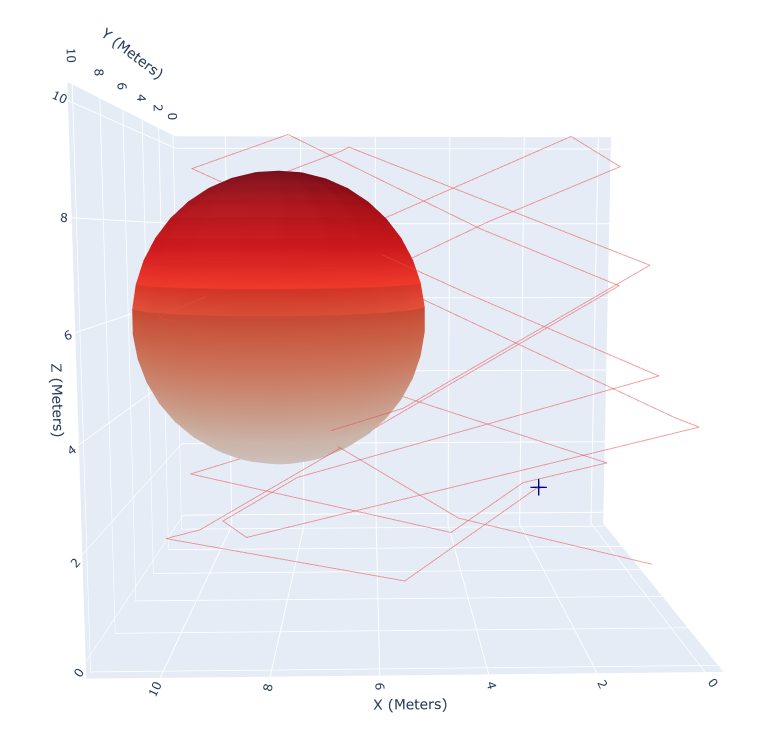
\includegraphics[width=0.8\textwidth]{kapitel4/3dplot3}
  \caption{Ein Strahl im interaktiven 3D Visualizer.}
  \label{fig:3dplot3}
\end{figure}

\subsection{Behandlung von Fließkomma-Ungenauigkeiten (Self-Intersection)}
\label{subsec:epsilon_fix}

Die Auswertung der Strahlengänge durch den Visualizer offenbarte ein kritisches algorithmisches Problem: Strahlen wurden unregelmäßig terminiert.
Die Ursache hierfür lag in der Fließkomma-Ungenauigkeit der CPU.
Wenn ein Strahlengang an einer Wand reflektiert wird, dient dieser mathematische Schnittpunkt als Ursprung für den nachfolgenden Reflexionsstrahl.
In der nächsten Iteration prüft die Engine den neuen Strahl gegen alle Wände, inklusive der Wand, auf der er sich bereits befindet.
Aufgrund von Rundungsfehlern berechnet der Algorithmus die Distanz zur aktuellen Wand nicht als $0{,}0$, sondern beispielsweise als $-0{,}0000001$.

\begin{figure}[htbp]
  \centering
  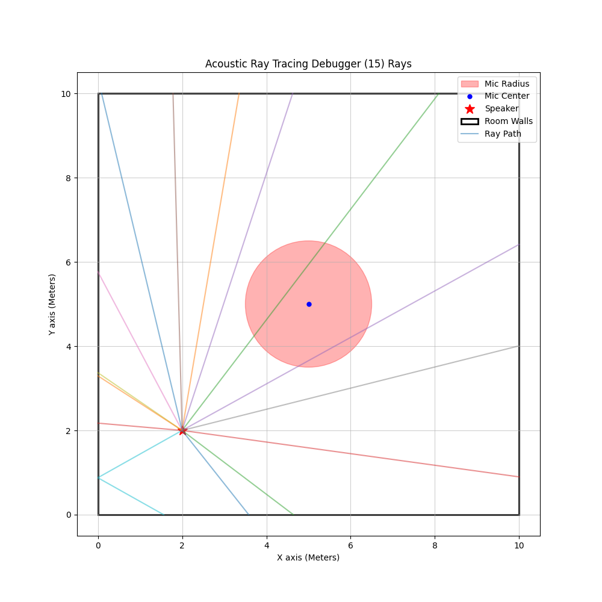
\includegraphics[width=0.8\textwidth]{kapitel4/shadowacne1}
  \caption{2D-Visualizer: Strahl reflektiert aufgrund von Rundungsfehlern auf derselben Wand.}
  \label{fig:shadowacne1}
\end{figure}

Die ursprüngliche Abbruchbedingung lautete: \texttt{if ray\_t < 0.0 \{ return None; \}}.
Da sehr kleine negative Fließkomma-Werte aufgrund von Präzisionsverlusten oft ignoriert oder fehlerhaft evaluiert wurden, registrierte die Engine fälschlicherweise sofortige, valide Treffer auf derselben Wand.
Der Strahl \enquote{reflektierte} in einer Endlosschleife am selben Punkt, bis das \texttt{max\_bounces}-Limit erschöpft war.
In der Computergrafik ist dieses Phänomen als \emph{Shadow Acne} bekannt.
Zur Lösung dieses Problems wurde ein Epsilon-Wert ($\epsilon$) eingeführt.
Die Bedingung wurde zu \texttt{if ray\_t < 0.001 \{ return None; \}} modifiziert.
Ein berechneter Schnittpunkt wird folglich nur als valide betrachtet, wenn der Strahl eine Mindestdistanz von $1\,\text{mm}$ zurückgelegt hat.
Die erneute Visualisierung bestätigte, dass das physikalische Verhalten nun korrekt simuliert wurde.

\begin{figure}[htbp]
  \centering
  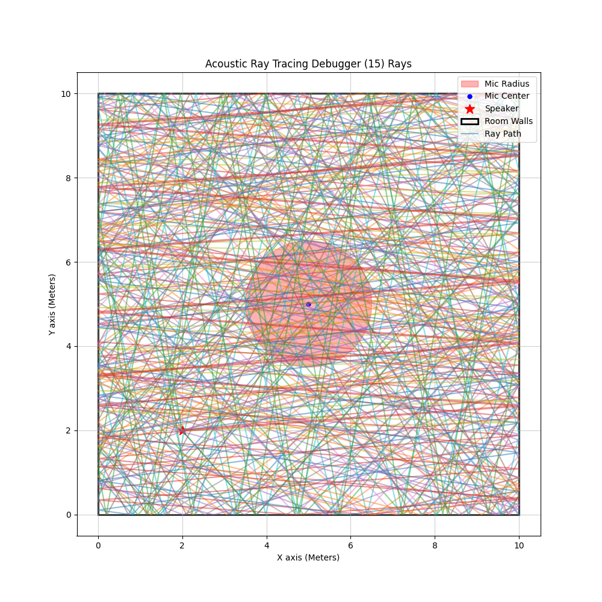
\includegraphics[width=0.8\textwidth]{kapitel4/fixedshadowacne}
  \caption{2D-Visualizer mit implementiertem Epsilon-Fix.}
  \label{fig:shadowacne2}
\end{figure}
  \newpage

% Ergaenzter Dokumentationsteil (aus der separaten Implementationsdoku)


% ========================================
\subsection{Themenschwerpunkt: Audio I/O und 3D-Raumdaten}
% ========================================

Dieser Abschnitt beschreibt die Implementierung zweier Komponenten des Multithreaded Acoustic Ray Tracers:

\begin{enumerate}
    \item \textbf{Audio I/O:} Einlesen trockener WAV-Dateien und Export des verarbeiteten, halligen Audio-Signals mit Clipping-Pr\"avention
    \item \textbf{Raumdaten:} Laden von 3D-Modellen aus \texttt{.obj}-Dateien und Konvertierung in das interne JSON-Format
\end{enumerate}

Die Implementierung erfolgt in Python und integriert sich nahtlos in die bestehende Pipeline, die Rust-basierte Physik-Engine, DSP-Convolution und Multithreading verbindet.

\subsection{Architektur-\"Ubersicht}

Das System folgt einer erweiterten Pipeline mit automatischer Raumgeometrie-Integration:

\begin{enumerate}
    \item[\textbf{[0/4]}] OBJ-Import: \texttt{room.obj} $\to$ \texttt{room\_geometry.json} mit Material-Absorption
    \item[\textbf{[1/4]}] Rust Physics Engine: L\"adt Raumgeometrie, simuliert Schallstrahlen, erzeugt IR
    \item[\textbf{[2/4]}] Audio-Einlesung: L\"adt trockene WAV-Datei
    \item[\textbf{[3/4]}] DSP-Convolution: Wendet IR mit frequenzabh\"angiger Material-D\"ampfung an
    \item[\textbf{[4/4]}] Audio-Export: Normalisiert und speichert Ergebnis
\end{enumerate}

Das Wandmaterial wird in \texttt{input\_config.json} konfiguriert und durchgehend durch alle Stufen propagiert: von der Geometrie-Absorption im Rust-Tracer bis zur oktavbandbasierten Frequenzformung in der Convolution.

% ========================================
\subsection{Audio I/O Handling}
% ========================================

\subsubsection{Anforderungen (Akzeptanzkriterien)}

\begin{enumerate}
    \item Sauberes Einlesen der \texttt{unprocessed.wav} ohne Qualit\"atsverlust
    \item Export der finalen WAV-Datei ohne Artefakte
    \item Normalisierung, damit geschichtetes Audio beim Export nicht clippt
\end{enumerate}

\subsection{Theoretischer Hintergrund}

\subsubsection{WAV-Format und Audio-Digitalisierung}

Das WAV-Format speichert Audiodaten als zeitdiskrete Samples mit konstanter Abtastfrequenz $f_s$:

$$x[n] = \int_{(n-0.5)/f_s}^{(n+0.5)/f_s} x_{\text{analog}}(t) \, dt$$

Jedes Sample liegt im Bereich $[-1.0, 1.0]$ (bei normalisierten 16/32-Bit PCM).

\subsubsection{WAV-Format: Technische Spezifikation}

Das WAV-Format (Waveform Audio File Format) speichert unkomprimierte PCM-Audiodaten
in einem RIFF-Container. Die f\"ur die Pipeline relevanten Parameter:

\begin{table}[H]
    \centering
    \begin{tabular}{|l|l|p{5cm}|}
        \hline
        \textbf{Parameter} & \textbf{Typische Werte} & \textbf{Bedeutung} \\
        \hline
        Abtastrate $f_s$ & 44.100\,Hz, 48.000\,Hz & Samples pro Sekunde \\
        \hline
        Bit-Tiefe & 16-bit, 24-bit, 32-bit float & Amplitude-Aufl\"osung \\
        \hline
        Kan\"ale & 1 (Mono), 2 (Stereo) & Anzahl unabh\"angiger Signale \\
        \hline
        Kodierung & PCM (Integer) oder IEEE Float & Speicherformat der Samples \\
        \hline
    \end{tabular}
    \caption{WAV-Formatparameter und ihre Bedeutung f\"ur die Pipeline}
\end{table}

Die \texttt{soundfile}-Bibliothek normalisiert beim Einlesen automatisch:
16-bit-Integer-Samples im Bereich $[-32768,\,32767]$ werden in \texttt{float64}-Werte
im Bereich $[-1.0,\,1.0]$ umgewandelt. Diese Skalierung ist verlustfrei -- die
Quantisierungsschritte des PCM-Formats bleiben erhalten. 32-bit-Float-WAV
wird direkt \"ubernommen. Die Pipeline erwartet stets Float-Daten; \texttt{write\_wav}
schreibt standardm\"a\ss{}ig 32-bit-Float zur\"uck, was f\"ur Hall-Anwendungen
bei $f_s = 44.100$\,Hz ausreicht.

\textbf{Abtastraten-Konsistenz:} Die Rust-Engine ist in \texttt{input\_config.json}
mit einer festen Abtastrate konfiguriert ($44.100$\,Hz).
Stimmt die Abtastrate der Eingangs-WAV nicht \"uberein, gibt die Pipeline eine Warnung aus
ohne automatisches Resampling, da eine Rateninkonsistenz alle Verzögerungen
der Impulsantwort um den Ratenquotienten staucht oder dehnt und den Hall
hörbar verstimmt.

\subsubsection{Clipping und Normalisierung}

Wenn w\"ahrend der Convolution (Faltung) die Amplitude $|y[n]|$ \"uber 1.0 steigt, tritt \textbf{Clipping} auf:

$$y_{\text{clipped}}[n] = \begin{cases}
    1.0 & \text{wenn } y[n] > 1.0 \\
    y[n] & \text{wenn } |y[n]| \leq 1.0 \\
    -1.0 & \text{wenn } y[n] < -1.0
\end{cases}$$

Um dies zu vermeiden, normalisieren wir:

$$y_{\text{norm}}[n] = \frac{y[n]}{A_{\max}} \quad \text{wobei} \quad A_{\max} = \max_n |y[n]|$$

Diese Normalisierung ist bewusst \textbf{konditional}: Liegt das Maximum bereits
unter 1.0, wird nicht skaliert da leise Signale nicht k\"unstlich lauter gemacht werden.
Die Pegelrelation zwischen verschiedenen Material-L\"aufen bleibt damit
erhalten, was akustische Vergleiche erm\"oglicht.

\subsection{Implementierung: \texttt{wav\_handler.py}}

\subsubsection{WAV-Einlesung}

\begin{lstlisting}
import numpy as np
import soundfile as sf

def read_wav(wav_path: str) -> tuple:
    """
    Reads a WAV file and returns the audio data as a NumPy array
    along with the corresponding sample rate.
    """
    audio_data, sample_rate = sf.read(wav_path)
    return audio_data, sample_rate
\end{lstlisting}

\textbf{Funktionsweise:}

\begin{itemize}
    \item Die \texttt{soundfile}-Bibliothek liest WAV-Dateien robust
    \item \texttt{audio\_data} ist ein NumPy-Array der Form \texttt{(samples,)} oder \texttt{(samples, channels)}
    \item \texttt{sample\_rate} ist die Abtastfrequenz in Hz
\end{itemize}

\subsubsection{WAV-Export mit Normalisierung}

\begin{lstlisting}
def write_wav(wav_path: str, audio_data, sample_rate: int) -> None:
    """
    Normalizes the audio data to prevent clipping and exports it to a WAV file.
    """
    max_amplitude = np.max(np.abs(audio_data))
    if max_amplitude > 1.0:
        audio_data = audio_data / max_amplitude
    sf.write(wav_path, audio_data, sample_rate)
\end{lstlisting}

\textbf{Algorithmus:}

\begin{algorithm}
    \caption{Normalisierter WAV-Export}
    \begin{algorithmic}
        \STATE $A_{\max} \gets \max_n |y[n]|$
        \IF{$A_{\max} > 1.0$}
            \STATE $y[n] \gets y[n] / A_{\max}$ f\"ur alle $n$
        \ENDIF
        \STATE Schreibe normalisierte Samples in WAV-Datei
    \end{algorithmic}
\end{algorithm}

\subsubsection{Integration in die Pipeline}

\begin{lstlisting}
# main.py Schritt [2/4]: Audio laden
dry_audio, sample_rate = read_wav(input_wav_path)

# Schritt [3/4]: Convolution mit Material-Absorption
conv_material = ir_data.get("metadata", {}).get("wall_material")
wet_audio = convolve(dry_audio, sample_rate, ir_data, material=conv_material)

# Schritt [4/4]: Normalisieren und exportieren
write_wav(output_wav_path, wet_audio, sample_rate)
\end{lstlisting}

Der \texttt{wall\_material}-Wert wird automatisch aus \texttt{ir\_output.json} gelesen, das der Rust-Tracer nach der Simulation schreibt. Damit nutzen Tracer und Convolution stets dasselbe Material.

% ========================================
\subsection{3D-Raumdaten: OBJ-Parser}
% ========================================

\subsubsection{Theoretischer Hintergrund}

\paragraph{OBJ-Format}

Das Wavefront \texttt{.obj}-Format ist ein textbasiertes 3D-Modellformat.
Jede Zeile beginnt mit einem Schl\"usselwort, das den Zeilentyp bestimmt:

\begin{lstlisting}[language={}]
# Vertices (Ecken)
v  1.0  2.0 -1.5    # Vertex 1
v  2.0  2.0 -1.5    # Vertex 2
v  1.0  3.0 -1.5    # Vertex 3

# Faces (Dreiecke, Format: v/vt/vn)
f  1/1/1  2/2/1  3/3/1  # Textur- und Normal-Indizes optional
\end{lstlisting}

Der Parser verarbeitet nur die f\"ur Raytracing relevanten Zeilen:

\begin{table}[H]
    \centering
    \begin{tabular}{|l|l|c|}
        \hline
        \textbf{Zeilentyp} & \textbf{Bedeutung} & \textbf{Verarbeitet?} \\
        \hline
        \texttt{v x y z} & Vertex-Position & \checkmark \\
        \hline
        \texttt{f v1 v2 v3} & Dreiecksfläche (Vertex-Indizes) & \checkmark \\
        \hline
        \texttt{f v/vt/vn} & Face mit Textur- und Normalindex & \checkmark (nur v) \\
        \hline
        \texttt{vn nx ny nz} & Vertex-Normale & Ignoriert \\
        \hline
        \texttt{vt u v} & Textur-Koordinate & Ignoriert \\
        \hline
        \texttt{usemtl name} & Material-Zuweisung (.mtl) & Ignoriert \\
        \hline
        \texttt{\#\ ...} & Kommentar & Ignoriert \\
        \hline
    \end{tabular}
    \caption{OBJ-Zeilentypen und Verarbeitungsstatus im Parser}
\end{table}

\textbf{Indexierung:} OBJ nutzt 1-basierte Indizes, Python 0-basierte.
Der Parser subtrahiert beim Einlesen automatisch 1.

\subsubsection{Dreiecks-Repr\"asentation}

$$\text{Triangle} = \begin{bmatrix}
x_1 & y_1 & z_1 \\
x_2 & y_2 & z_2 \\
x_3 & y_3 & z_3
\end{bmatrix}$$

\subsection{Implementierung: \texttt{obj\_parser.py}}

\subsubsection{OBJ-Loader}

\begin{lstlisting}
def load_obj_to_triangles(file_path: str) -> list:
    vertices = []
    triangles = []
    path = Path(file_path)
    if not path.exists():
        raise FileNotFoundError(f"The 3D file '{file_path}' was not found.")
    with path.open('r') as f:
        for line in f:
            line = line.strip()
            if line.startswith('v '):
                parts = line.split()
                x, y, z = float(parts[1]), float(parts[2]), float(parts[3])
                vertices.append([x, y, z])
            elif line.startswith('f '):
                parts = line.split()
                v1_idx = int(parts[1].split('/')[0]) - 1
                v2_idx = int(parts[2].split('/')[0]) - 1
                v3_idx = int(parts[3].split('/')[0]) - 1
                triangle = [vertices[v1_idx], vertices[v2_idx], vertices[v3_idx]]
                triangles.append(triangle)
    return triangles
\end{lstlisting}

\subsubsection{Material-basierter Export: \texttt{export\_room\_geometry()}}

Die neue Exportfunktion verbindet OBJ-Geometrie mit der Materialdatenbank
(\texttt{materials.json}) und schreibt \texttt{room\_geometry.json} f\"ur den Rust-Tracer.
Jedes Dreieck erh\"alt die mittlere Absorptionskonstante des gew\"ahlten Materials:

\begin{lstlisting}
_MATERIALS_JSON = Path(__file__).resolve().parent.parent / "rust_service" / "materials.json"

def _mean_absorption(material: str) -> float:
    """Mittlere Absorption aus materials.json fuer das gewaehlte Material."""
    data = json.loads(_MATERIALS_JSON.read_text())
    alphas = data["materials"][material]["absorption"]
    return sum(alphas) / len(alphas)

def export_room_geometry(obj_path: str, material: str, out_path: str) -> None:
    triangles_raw = load_obj_to_triangles(obj_path)
    absorption = _mean_absorption(material)
    triangles = [
        {"v0": t[0], "v1": t[1], "v2": t[2], "absorption": absorption}
        for t in triangles_raw
    ]
    out = {"triangles": triangles, "triangle_count": len(triangles)}
    Path(out_path).write_text(json.dumps(out, indent=2))
\end{lstlisting}

\subsubsection{Ausgabeformat: \texttt{room\_geometry.json}}

Der Rust-Tracer liest Dreiecke inkl.\ Material-Absorption aus dieser Datei:

\begin{lstlisting}[language={}]
{
  "triangles": [
    {"v0": [0.0, 0.0, 0.0], "v1": [12.0, 0.0, 0.0],
     "v2": [12.0, 12.0, 0.0], "absorption": 0.033}
  ],
  "triangle_count": 12
}
\end{lstlisting}

Die \texttt{absorption}-Werte entsprechen dem arithmetischen Mittel aller 6 Oktavb\"ander
aus \texttt{materials.json}. Die frequenzabh\"angige Verarbeitung findet ausschlie\ss{}lich
in der Python-Convolution statt.

\subsection{Blender-Workflow: Raum erstellen und exportieren}

F\"ur realistische Raumakustik kann jede beliebige Raumgeometrie aus Blender
exportiert werden. Der empfohlene Workflow:

\begin{enumerate}
    \item \textbf{Raum modellieren}: Geschlossenen Raum in Blender erstellen.
    Alle Fl\"achen m\"ussen nach innen zeigen (\textit{Face Normals} pr\"ufen).
    \item \textbf{Triangulieren}: \textit{Edit Mode} $\to$ \textit{Mesh} $\to$
    \textit{Faces} $\to$ \textit{Triangulate Faces} (Shortcut: \texttt{Ctrl+T}).
    Der OBJ-Parser verarbeitet ausschlie\ss{}lich Dreiecke.
    \item \textbf{Exportieren}: \textit{File} $\to$ \textit{Export} $\to$
    \textit{Wavefront (.obj)}
    \begin{itemize}
        \item Koordinatensystem: Y Forward, Z Up (passend zu \texttt{input\_config.json})
        \item Haken bei \textit{Triangulate Mesh} setzen
        \item Speichern als \texttt{room.obj} in \texttt{python\_service/}
    \end{itemize}
    \item \textbf{Positionen pr\"ufen}: Speaker- und Mic-Positionen in
    \texttt{input\_config.json} m\"ussen innerhalb des Modells liegen.
    Die Mic-Position zuz\"uglich \texttt{mic\_radius} darf keine Wand \"uberschreiten.
    \item \textbf{Pipeline starten}: \texttt{python main.py} erkennt \texttt{room.obj}
    automatisch und generiert \texttt{room\_geometry.json} vor dem Rust-Lauf.
\end{enumerate}

% ========================================
\subsection{Integration und Testing}
% ========================================

\subsubsection{End-to-End-Pipeline}

Die Pipeline verl\"auft nun in 5 Schritten. Schritt~0 ist vollautomatisch:
\texttt{room.obj} wird erkannt, mit dem konfigurierten Material in
\texttt{room\_geometry.json} umgewandelt und dem Rust-Tracer bereitgestellt.

\begin{lstlisting}
# Schritt 0: OBJ -> room_geometry.json (automatisch wenn room.obj vorhanden)
if Path("room.obj").exists():
    export_room_geometry("room.obj", wall_material,
                         "../rust_service/room_geometry.json")

# Schritt 1: Rust Physics Engine
ir_data = run_rust_and_load_json(rust_binary_path, json_path)

# Schritt 2: Audio laden
dry_audio, sample_rate = read_wav(input_wav_path)

# Schritt 3: Convolution mit Material-Absorption
conv_material = ir_data.get("metadata", {}).get("wall_material")
wet_audio = convolve(dry_audio, sample_rate, ir_data, material=conv_material)

# Schritt 4: Normalisieren und exportieren
write_wav(output_wav_path, wet_audio, sample_rate)
\end{lstlisting}

\subsection{Material-Konfiguration}

Das Wandmaterial wird in \texttt{rust\_service/materials.json} festgelegt:

\begin{lstlisting}[language={}]
"materials": {
    "concrete": {
      "absorption": [0.02, 0.03, 0.03, 0.03, 0.04, 0.07],
      "scattering": 0.05
    },
\end{lstlisting}

Vom Rust-Tracer wird \texttt{wall\_material} in \texttt{ir\_output.json} exportiert
und von der Python-Pipeline automatisch f\"ur die Convolution \"ubernommen.
Verf\"ugbare Materialien (aus \texttt{materials.json}):

\begin{table}[H]
    \centering
    \begin{tabular}{|l|l|c|}
        \hline
        \textbf{Material} & \textbf{Beschreibung} & \textbf{Mittl. Absorption} \\
        \hline
        \texttt{concrete} & Beton  & 0.033 \\
        \hline
        \texttt{wood}  & Holz & 0.11 \\
        \hline
        \texttt{glass}    & Glas  & 0.026 \\
        \hline
        \texttt{carpet}   & Teppich  & 0.425 \\
        \hline
    \end{tabular}
    \caption{Verf\"ugbare Materialien in \texttt{materials.json}}
\end{table}

\subsection{Konfiguration: \texttt{input\_config.json}}

Alle Simulationsparameter werden in einer einzigen JSON-Datei geb\"undelt,
die sowohl vom Rust-Tracer als auch von der Python-Pipeline gelesen wird:

\begin{table}[H]
    \centering
    \begin{tabular}{|l|l|p{5.5cm}|}
        \hline
        \textbf{Feld} & \textbf{Beispielwert} & \textbf{Bedeutung} \\
        \hline
        \texttt{speaker\_position} & \texttt{[2.0, 3.0, 1.5]} & 3D-Position der Schallquelle \\
        \hline
        \texttt{mic\_position} & \texttt{[8.0, 7.0, 6.0]} & 3D-Position des Mikrofons \\
        \hline
        \texttt{mic\_radius} & \texttt{3.0} & Einfangradius des Mikrofons in Metern \\
        \hline
        \texttt{rays\_to\_cast} & \texttt{1000} & Anzahl der simulierten Strahlen \\
        \hline
        \texttt{max\_bounces} & \texttt{100} & Max.\ Reflexionen pro Strahl \\
        \hline
        \texttt{min\_pressure} & \texttt{0.001} & Abbruchschwelle (Restdruck) \\
        \hline
        \texttt{wall\_material} & \texttt{"concrete"} & Wandmaterial (aus \texttt{materials.json}) \\
        \hline
    \end{tabular}
    \caption{Felder der \texttt{input\_config.json}}
\end{table}

Das Feld \texttt{wall\_material} wird von der Python-Pipeline beim
Start ausgelesen, um \texttt{room\_geometry.json} mit der passenden Absorption
zu generieren. Der Rust-Tracer schreibt es anschlie\ss{}end in \texttt{ir\_output.json},
von wo die Convolution es f\"ur die frequenzabh\"angige D\"ampfung \"ubernimmt.



% ========================================
\subsection{Visualisierung: \texttt{visualizer.py}}
% ========================================

\subsection{\"Ubersicht}

Der Visualizer rendert die Ergebnisse der Rust-Simulation als interaktive
3D-Szene im Browser (Plotly). Er liest zwei Dateien aus dem \texttt{rust\_service}:

\begin{itemize}
    \item \texttt{visualisation\_data.json}: Strahlpfade, Speaker- und Mic-Position
    \item \texttt{room\_geometry.json}: Raumw\"ande als Dreiecksliste (optional)
\end{itemize}

\subsection{Raumwände-Rendering}

Die Funktion \texttt{\_draw\_room\_walls()} wurde neu implementiert und l\"adt
\texttt{room\_geometry.json}, falls vorhanden, und zeichnet jedes Dreieck als
blaues Drahtgitter:

\begin{lstlisting}
def _draw_room_walls(fig: go.Figure, geometry_path: Path) -> None:
    if not geometry_path.exists():
        return
    data = json.loads(geometry_path.read_text())
    for tri in data["triangles"]:
        v0, v1, v2 = tri["v0"], tri["v1"], tri["v2"]
        xs = [v0[0], v1[0], v2[0], v0[0]]
        ys = [v0[1], v1[1], v2[1], v0[1]]
        zs = [v0[2], v1[2], v2[2], v0[2]]
        fig.add_trace(go.Scatter3d(
            x=xs, y=ys, z=zs, mode='lines',
            line=dict(width=1, color='rgba(100,130,200,0.35)'),
            showlegend=False, hoverinfo='skip'))
\end{lstlisting}

Durch das R\"uckschlie\ss{}en des Dreiecks (\texttt{v0} als vierter Punkt) entsteht
ein geschlossenes Dreieck. Die halbtransparente Farbe \texttt{rgba(100,130,200,0.35)}
h\"alt die Raumw\"ande visuell im Hintergrund, sodass die Strahlpfade im Vordergrund
bleiben.

\subsection{Dargestellte Elemente}

\begin{table}[H]
    \centering
    \begin{tabular}{|l|l|l|}
        \hline
        \textbf{Element} & \textbf{Darstellung} & \textbf{Datenquelle} \\
        \hline
        Strahlpfade & Farbige Linien (Golden-Angle-Farbfolge) & \texttt{visualisation\_data.json} \\
        \hline
        Lautsprecher & Blauer Kreuz-Marker & \texttt{visualisation\_data.json} \\
        \hline
        Mikrofon-Zentrum & Blauer Punkt & \texttt{visualisation\_data.json} \\
        \hline
        Mikrofon-Radius & Rote Kugel (halbtransparent) & \texttt{visualisation\_data.json} \\
        \hline
        Raumw\"ande & Hellblaues Drahtgitter & \texttt{room\_geometry.json} \\
        \hline
    \end{tabular}
    \caption{Visuelle Elemente der 3D-Debugging-Szene}
\end{table}

Die Golden-Angle-Farbfolge $\varphi_i = (i \cdot 137{,}5\,\%) \bmod 360$
verteilt die Strahlfarben gleichm\"a\ss{}ig im HSL-Farbraum, sodass auch bei
vielen Strahlen kein Farbton doppelt vorkommt.

\subsection{Starten des Visualizers}

\begin{lstlisting}[language=bash]
cd python_service
python visualizer.py
\end{lstlisting}

Plotly \"offnet automatisch einen Browser-Tab mit der interaktiven 3D-Szene.
Fehlt \texttt{room\_geometry.json}, werden keine Raumw\"ande gezeichnet;
die Datei wird durch Ausf\"uhren der Pipeline mit einer \texttt{room.obj} erzeugt.

% ========================================
\subsection{Akzeptanzkriterien und Validierung}
% ========================================

\subsubsection{Audio I/O}

\begin{table}[H]
    \centering
    \begin{tabular}{|p{4.5cm}|p{2cm}|p{5cm}|}
        \hline
        \textbf{Kriterium} & \textbf{Erf\"ullt?} & \textbf{Test} \\
        \hline
        Sauberes Einlesen .wav & \checkmark & \texttt{len(audio\_data) > 0} \\
        \hline
        Export ohne Qualit\"atsverlust & \checkmark & H\"ortest, Spektrum-Analyse \\
        \hline
        Normalisierung gegen Clipping & \checkmark & \texttt{max(abs(audio)) <= 1.0} \\
        \hline
    \end{tabular}
\end{table}

\subsubsection{Raumdaten: OBJ-Parser \& Material-Integration}

\begin{table}[H]
    \centering
    \begin{tabular}{|p{4.5cm}|p{2cm}|p{5cm}|}
        \hline
        \textbf{Kriterium} & \textbf{Erf\"ullt?} & \textbf{Test} \\
        \hline
        Parser liest .obj & \checkmark & \texttt{len(triangles) > 0} \\
        \hline
        JSON-Export mit Absorption & \checkmark & \texttt{absorption}-Feld pro Dreieck \\
        \hline
        Rust l\"adt OBJ-Geometrie & \checkmark & \texttt{room\_geometry.json} erkannt \\
        \hline
        Material durchgereicht & \checkmark & \texttt{wall\_material} in \texttt{ir\_output.json} \\
        \hline
        Frequenzabh\"ang. Convolution & \checkmark & \texttt{apply\_material\_absorption()} \\
        \hline
    \end{tabular}
\end{table}

\subsection{Materialvergleich: Akustisches Verhalten}

Die folgende Tabelle zeigt das Verhalten der Pipeline mit dem Test-Raum
(12\,m $\times$ 12\,m $\times$ 10\,m, 100 Strahlen, 100 maximale Bounces):

\begin{table}[H]
    \centering
    \begin{tabular}{|l|c|c|p{5cm}|}
        \hline
        \textbf{Material} & \textbf{Hits} & \textbf{Eff. Bounces} & \textbf{Klangcharakter} \\
        \hline
        \texttt{concrete} & $\sim$2000 & bis 100 & Hell, langer Nachhall (Kathedrale) \\
        \hline
        \texttt{glass}    & $\sim$2200 & bis 100 & Sehr hell, extrem langer Nachhall \\
        \hline
        \texttt{drywall}  & $\sim$1500 & $\sim$43 & Moderat, typischer Wohnraum \\
        \hline
        \texttt{carpet}   & $\sim$400  & $\sim$11 & Dumpf, kurzer Nachhall \\
        \hline
        \texttt{foam}     & $\sim$200  & $\sim$7  & Sehr trocken, fast kein Nachhall \\
        \hline
    \end{tabular}
    \caption[Verhalten verschiedener Materialien]{Verhalten verschiedener Materialien (Richtwerte, 12\,m\,$\times$\,12\,m\,$\times$\,10\,m Testraum)}
\end{table}

Die \textbf{effektiven Bounces} ergeben sich aus der Bedingung
$(1 - \alpha)^n < p_{\min}$ mit $p_{\min} = 0.001$:
$n < \ln(0.001) / \ln(1 - \alpha)$.
Bei Beton ($\alpha = 0.033$) ben\"otigt ein Strahl theoretisch 204 Bounces,
wird aber durch \texttt{max\_bounces = 100} begrenzt.
Bei Teppich ($\alpha = 0.425$) bricht er bereits nach 11 Bounces ab.












